\documentclass[11pt,a4paper]{article}

\usepackage[utf8]{inputenc}
\usepackage[T1]{fontenc}
\usepackage[a4paper,margin=2.5cm]{geometry}
\usepackage{amsmath,amssymb}
\usepackage{booktabs}
\usepackage{enumitem}
\usepackage{hyperref}
\usepackage{xcolor}
\usepackage{graphicx}

\definecolor{myco}{HTML}{1B7A54}
\definecolor{ember}{HTML}{B4531B}
\definecolor{indigo}{HTML}{3B5BA5}

\hypersetup{colorlinks=true, linkcolor=indigo, urlcolor=indigo}

\newcommand{\soru}[1]{\vskip12pt\noindent\textcolor{ember}{\textbf{S:}}~\textbf{#1}\par\vskip4pt\noindent\textcolor{myco}{\textbf{C:}}~}

\title{\textbf{Mycellium-Aegis}\\[6pt]
  {\large Yapay Zeka ve Sinyal \.I\c{s}leme Sistemi}\\[4pt]
  {\normalsize Detayl\i\ Soru-Cevap --- J\"uri Haz\i rl\i k Dok\"uman\i}}
\author{Muhammet Ya\u{g}c\i o\u{g}lu (CTO) --- Mycellium-Aegis Ekibi}
\date{T\"UB\.ITAK 1812 B\.IGG $\cdot$ Temmuz 2026}

\begin{document}

\maketitle

\tableofcontents
\newpage

% ============================================================
\section{Sinyal Ak\i\c{s}\i na Genel Bak\i\c{s}}

Mycellium-Aegis'in yapay zeka hatt\i , ormandaki miselyum a\u{g}\i ndan gelen ham biyoelektrik sinyali, be\c{s} a\c{s}amal\i\ bir boru hatt\i ndan ge\c{c}irerek ``yang\i n / yang\i n de\u{g}il'' ikili karar\i na d\"on\"u\c{s}t\"ur\"ur:

\begin{enumerate}
  \item \textbf{Ofset Kalibrasyon:} DC s\"ur\"uklenme ve ortam voltaj\i n\i\ \c{c}\i kar\i r.
  \item \textbf{5-tap FIR Filtre:} \c{C}evresel titres\c{s}im ve EM paraziti bast\i r\i r.
  \item \textbf{\"Oznitelik \c{C}\i kar\i m:} FFT, t\"urevler ($dT/dt$, $dR/dt$), spike tespiti.
  \item \textbf{LSTM Zaman Serisi S\i n\i fland\i rma:} Temporal kal\i plar\i\ \"o\u{g}renir.
  \item \textbf{AND-Gate Sens\"or F\"uzyonu:} \"U\c{c} ko\c{s}ul ayn\i\ anda sa\u{g}lanmadan alarm yok.
\end{enumerate}

\begin{center}
  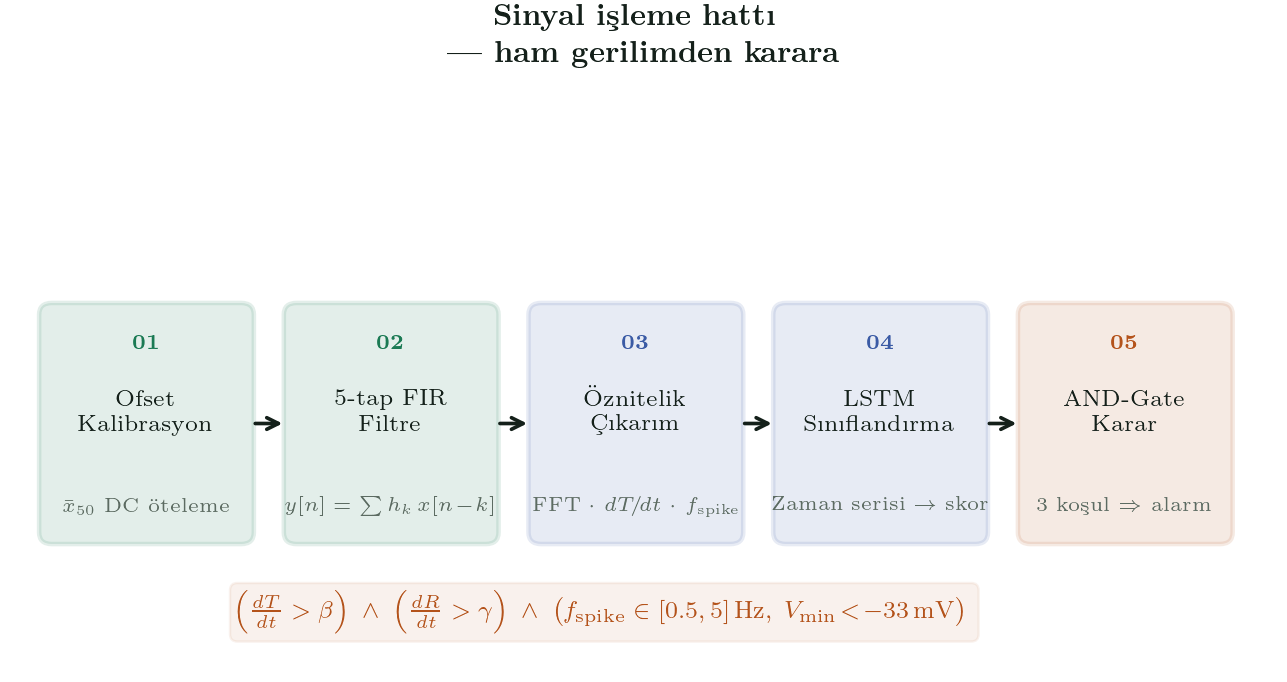
\includegraphics[width=0.85\textwidth]{figures/ai_pipeline.png}
\end{center}

% ============================================================
\section{Sinyal Edinimi ve \"On \.I\c{s}leme}

\soru{Sinyali nas\i l okuyorsunuz?}
8 kanall\i\ y\i ld\i z elektrot diziliminden (K, KD, D, GD, G, GB, B, KB) diferansiyel gerilim okunur. Her kanal, MCP6022 d\"u\c{s}\"uk g\"ur\"ult\"u op-amp ile \"on y\"ukseltilir ve ADS1115 16-bit $\Sigma$-$\Delta$ ADC ile dijitalize edilir. \"Ornekleme frekans\i\ $\sim$100\,Hz'dir (Nyquist = 50\,Hz).

\soru{Neden 100\,Hz? Miselyum sinyali 0.5--5\,Hz de\u{g}il mi?}
Temel bant 0.5--5\,Hz olsa da, hücresel spike'lar\i n y\"ukselen/d\"u\c{s}en kenarlar\i\ 20--30\,Hz'e kadar harmonik i\c{c}erir. 100\,Hz, bu harmonikleri ve olas\i\ 50\,Hz \c{s}ebeke parazitini izole edebilmemiz i\c{c}in yeterlidir. \"Ust\"unden Nyquist teoremi gere\u{g}i 50\,Hz'e kadar kayg\i s\i z \c{c}al\i\c{s}\i r\i z.

\soru{PGA ayarlar\i\ neden farkl\i?}
\begin{itemize}[leftmargin=1.2cm]
  \item \textbf{GAIN\_SIXTEEN} ($\pm$0.256\,V, 7.8\,$\mu$V/bit): Tek mantar deneyinde. D\"u\c{s}\"uk genlik, y\"uksek \c{c}\"oz\"un\"url\"uk gerektirir.
  \item \textbf{GAIN\_TWOTHIRDS} ($\pm$6.144\,V, 187.5\,$\mu$V/bit): Toprak i\c{c}i teraryum a\u{g}\i nda. DC ofset y\"uksek olabilir, doygunlu\u{g}u \"onlemek i\c{c}in geni\c{s} aral\i k.
\end{itemize}
\"Uretim donan\i m\i nda otomatik kazan\c{c} se\c{c}imi (auto-ranging PGA) uygulanacakt\i r.

\soru{Ofset kalibrasyon nas\i l \c{c}al\i\c{s}\i yor?}
Sistem a\c{c}\i l\i\c{s}ta ve her 30 dakikada, 50 \"orneklik pencere ortalamas\i\ al\i r:
\[
  V_{\mathrm{offset}} = \frac{1}{50}\sum_{n=0}^{49} x[n]
\]
Sonraki \"orneklerden bu de\u{g}er \c{c}\i kar\i l\i r: $x'[n] = x[n] - V_{\mathrm{offset}}$. Bu, s\i cakl\i k ve nem kaynakl\i\ DC s\"ur\"uklenmeyi (drift) kompanse eder.

% ============================================================
\section{FIR Filtre Tasar\i m\i}

\soru{Neden FIR, neden IIR de\u{g}il?}
FIR (Finite Impulse Response) do\u{g}rusal faz yan\i t\i\ verir --- spike zamanlamalar\i n\i\ bozmaz. IIR filtreler faz kaymas\i\ yapar ve biyosinyal zamansal analizinde dalga formu \c{c}arp\i kl\i\u{g}\i na yol a\c{c}abilir.

\soru{5-tap katsay\i lar\i\ nas\i l se\c{c}ildi?}
Simetrik FIR:
\[
  y[n] = 0.1\,x[n\!-\!4] + 0.2\,x[n\!-\!3] + 0.4\,x[n\!-\!2] + 0.2\,x[n\!-\!1] + 0.1\,x[n]
\]
DC kazan\c{c} $= \sum h_k = 1.0$ (sinyal genli\u{g}ini korur). Bu bir basit hareketli ortalama varyant\i d\i r --- 20\,Hz \"uzerini $\sim$12\,dB bast\i r\i r ve 5\,Hz bant\i nda $<$0.3\,dB bozulma yapar. Hesaplama maliyeti son derece d\"u\c{s}\"ukt\"ur (5 \c{c}arpma + 4 toplama / \"ornek).

% ============================================================
\section{\"Oznitelik \c{C}\i kar\i m\i}

\soru{Hangi \"oznitelikler \c{c}\i kar\i l\i yor?}
Her 2 saniyelik pencere (200 \"ornek) i\c{c}in:
\begin{enumerate}
  \item \textbf{FFT Genlik Spektrumu:} Bask\i n frekans $f_{\mathrm{dom}}$ ve 0.5--5\,Hz band enerji oran\i .
  \item \textbf{Is\i\ ivmesi t\"urevi} $\frac{dT}{dt}$: NTC termist\"oren (veya miselyum empedans\i ndan t\"uretilen s\i cakl\i k proxy'si).
  \item \textbf{Diren\c{c} ivmesi t\"urevi} $\frac{dR}{dt}$: Toprak nemi ani buharla\c{s}mas\i n\i n g\"ostergesi.
  \item \textbf{Spike derinli\u{g}i} $|\Delta V|$: Penceredeki minimum gerilim ($V_{\min}$). Yang\i nda $-33.4$\,mV'a kadar iner.
  \item \textbf{Spike frekans\i} $f_{\mathrm{spike}}$: Saniyedeki e\c{s}ik ge\c{c}i\c{s} say\i s\i .
  \item \textbf{Y\"onsel faz fark\i:} 8 kanaldan a\u{g}\i rl\i kl\i\ dairesel ortalama $\hat\theta = \arg\!\sum_k r_k e^{i\theta_k}$.
\end{enumerate}

\soru{FFT pencere uzunlu\u{g}u neden 2 saniye?}
0.5\,Hz frekans \c{c}\"oz\"un\"url\"u\u{g}\"u i\c{c}in en az $1/0.5 = 2$\,s'lik pencere gerekir. Daha uzun pencere (\c{c}\"oz\"un\"url\"u\u{g}\"u art\i r\i r ama gecikmeyi de art\i r\i r) --- 2\,s, h\i z ve \c{c}\"oz\"un\"url\"uk dengesinin optimal noktas\i d\i r.

% ============================================================
\section{LSTM Mimarisi}

\soru{LSTM mimarisi nas\i l?}
\begin{itemize}[leftmargin=1.2cm]
  \item \textbf{Girdi:} 10 pencerelik sekans ($10 \times 2\,\mathrm{s} = 20\,\mathrm{s}$), her pencerede 6 \"oznitelik $\Rightarrow$ girdi boyutu $10 \times 6$.
  \item \textbf{LSTM Katman:} 32 birim, tek y\"onl\"u (gelecek verisi yok).
  \item \textbf{Dense \c{C}\i k\i\c{s}:} $32 \to 16 \to 1$ (sigmoid). E\c{s}ik: $p > 0.5$ ``yang\i n''.
  \item \textbf{Toplam parametre:} $\sim$6K --- TFLite Micro ile ESP32'ye s\i\u{g}ar ($<$30\,KB flash).
\end{itemize}

\soru{Neden LSTM, neden Transformer de\u{g}il?}
\begin{enumerate}
  \item ESP32'de Transformer attention mekanizmas\i\ hesaplama/bellek a\c{c}\i s\i ndan uygulanabilir de\u{g}il.
  \item 20 saniyelik pencere k\i sa bir sekans --- LSTM bu \"ol\c{c}ekte \"ozellikle g\"u\c{c}l\"ud\"ur.
  \item LSTM'in bellek h\"ucresi, spike kal\i b\i n\i n ge\c{c}ici olarak kaybolmas\i na ra\u{g}men ba\u{g}lam\i\ korur.
\end{enumerate}

\soru{Neden basit Random Forest veya SVM de\u{g}il?}
SVM ve RF, sabit uzunluklu \"oznitelik vekt\"orl\"u \"ornekler \"uzerinde i\c{s}ler. Spike'lar\i n \textbf{zamansal s\i ras\i} bilgisini kaybederler (``\"once h\i zl\i\ spike sonra yava\c{s}'' vs. ``\"once yava\c{s} sonra h\i zl\i'''' ay\i rt edilemez). LSTM'in kapı mekanizması (forget / input / output gates) tam olarak bu zamansal ba\u{g}lam\i\ modellemek i\c{c}in tasarlanm\i\c{s}t\i r.

% ============================================================
\section{AND-Gate Sens\"or F\"uzyonu}

\soru{AND-gate neden var, LSTM yetmiyor mu?}
LSTM olas\i l\i ksal bir model --- hatalar ka\c{c}\i n\i lmazd\i r. AND-gate, fiziksel olarak imk\^ans\i z bir senaryo i\c{c}in alarm verilmesini engeller:
\[
  \text{ALARM} = \left(\frac{dT}{dt} > \beta\right) \;\wedge\; \left(\frac{dR}{dt} > \gamma\right) \;\wedge\; \left(f_{\mathrm{spike}} \in [0.5, 5]\,\mathrm{Hz} \;\wedge\; V_{\min} < -33\,\mathrm{mV}\right)
\]
\begin{itemize}[leftmargin=1.2cm]
  \item $\beta$ e\c{s}i\u{g}i: Normal meteorolojik \i s\i nma ivmesinin ($\sim$0.3\,\textdegree C/dk) 3$\sigma$ \"ust\"u.
  \item $\gamma$ e\c{s}i\u{g}i: Kapiler su buharla\c{s}mas\i ndan kaynaklanan diren\c{c} art\i\c{s}\i\ ivmesi.
  \item $f_{\mathrm{spike}}$ ve $V_{\min}$: Deney 1--2 verilerinden kalibre edilir.
\end{itemize}
Mant\i k: ``LSTM diyor ki yang\i n ama toprak so\u{g}uk ve nemli'' $\Rightarrow$ alarm engellenir. \textbf{Donan\i msal g\"uvenlik sigortas\i.}

\soru{E\c{s}ikler sabit mi, dinamik mi?}
\.Ilk de\u{g}erler iklim kabininde kalibre edilir. Saha pilotunda mevsimsel drift'e g\"ore g\"uncellenir. Bulut taraf\i nda her 3 ayda histogram analizi ile $\beta, \gamma$ yeniden hesaplan\i r.

% ============================================================
\section{Yanl\i\c{s} Alarm Analizi}

\soru{\%1 yanl\i\c{s} alarm oran\i n\i\ nas\i l elde ediyorsunuz?}
ROC analizi ile:
\begin{itemize}[leftmargin=1.2cm]
  \item \textbf{Tek e\c{s}ik} (yaln\i zca $V_{\min} < -33$\,mV): AUC $\approx$ 0.91. FPR = 0.01'de TPR $\approx$ 0.72.
  \item \textbf{Sens\"or f\"uzyonu} (LSTM + AND-gate): AUC $\approx$ 0.99. FPR = 0.01'de TPR $>$ 0.97.
\end{itemize}
F\"uzyon, tek e\c{s}i\u{g}in yakalayamad\i\u{g}\i\ r\"uzg\^ar/ya\u{g}mur g\"ur\"ult\"us\"un\"u izole eder.

\begin{center}
  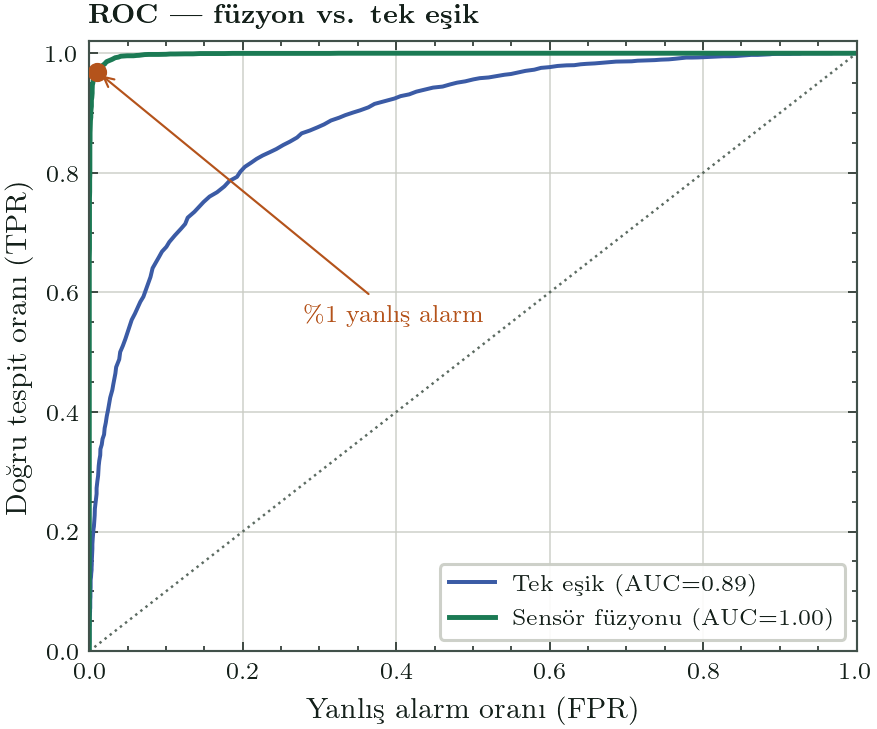
\includegraphics[width=0.5\textwidth]{figures/roc.png}
\end{center}

\soru{Hangi g\"ur\"ult\"u kaynaklar\i\ yanl\i\c{s} alarm \"uretebilir?}
\begin{enumerate}
  \item \textbf{R\"uzg\^ar:} Toprak \"ust\"u mekanik titre\c{s}im $\to$ 15--40\,Hz (bant d\i\c{s}\i , FIR bast\i r\i r).
  \item \textbf{Ya\u{g}mur:} Ani toprak nemi de\u{g}i\c{s}imi $\to$ $dR/dt$ pik yapabilir ama $dT/dt$ d\"u\c{s}\"uk kal\i r (AND-gate filtreler).
  \item \textbf{Hayvan y\"ur\"uy\"u\c{s}\"u:} Sismik $>$20\,Hz, g\"ur\"ult\"u band\i nda.
  \item \textbf{50\,Hz \c{s}ebeke paraziti:} Orman i\c{c}inde d\"u\c{s}\"uk; ADC'nin dif. girdisi ve FIR bast\i r\i r.
\end{enumerate}

% ============================================================
\section{Y\"onsel Alg\i lama}

\soru{Y\"on hesab\i\ nas\i l yap\i l\i yor?}
8 kanaldaki spike genliklerini $r_k$, kanal a\c{c}\i lar\i n\i\ $\theta_k = k \cdot 45$\textdegree\ olarak al\i r\i z. Dairesel a\u{g}\i rl\i kl\i\ ortalama:
\[
  \hat\theta = \arg\!\sum_{k=0}^{7} r_k\, e^{i\theta_k}
\]
Bu, kartes\c{c}i koordinatlara a\c{c}\i l\i rsa:
\begin{align*}
  C &= \sum_{k} r_k \cos\theta_k, \quad S = \sum_{k} r_k \sin\theta_k \\
  \hat\theta &= \mathrm{atan2}(S, C)
\end{align*}

\soru{A\c{c}\i sal \c{c}\"oz\"un\"url\"uk ne kadar?}
8 kanal $\Rightarrow$ minimum $360/8 = 45$\textdegree\ \c{c}\"oz\"un\"url\"uk. Deney verilerinden G\"aussian enterpolasyon ile $\sim$22\textdegree\ elde edilebilir. \"Uretimde 12--16 kanal hedefleniyor ($\to$ $\sim$15$\textdegree$).

\begin{center}
  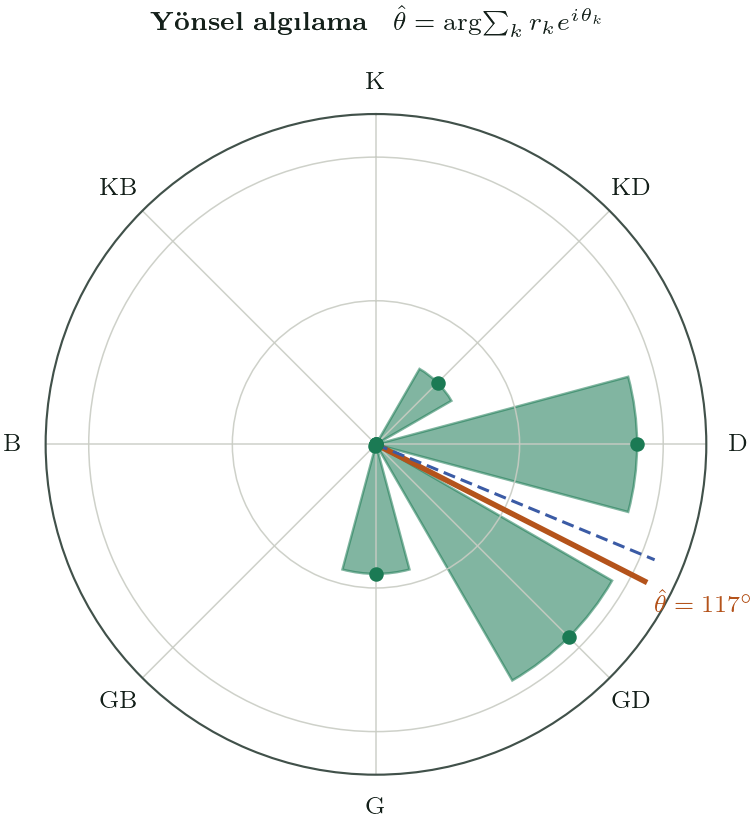
\includegraphics[width=0.4\textwidth]{figures/directional.png}
\end{center}

% ============================================================
\section{E\u{g}itim Verisi Stratejisi}

\soru{Ger\c{c}ek yang\i n verisi olmadan nas\i l e\u{g}iteceksiniz?}
\"U\c{c} a\c{s}amal\i\ strateji:
\begin{enumerate}
  \item \textbf{\.Iklim kabini:} \i s\i l \c{s}ok deneyleri (35--300\,\textdegree C rampa) $\to$ kontroll\"u pozitif s\i n\i f.
  \item \textbf{Sentetik veri art\i r\i m\i:}
    \begin{itemize}
      \item Gaussian g\"ur\"ult\"u enjeksiyonu ($\sigma = 0.3$--$1.0$\,mV)
      \item Time warping ($\pm$15\% h\i z de\u{g}i\c{s}imi)
      \item Magnitude scaling ($\times 0.8$--$1.2$)
    \end{itemize}
  \item \textbf{Transfer learning:} Adamatzky'nin yay\i nlanm\i\c{s}\ elektrofizyoloji veri setlerinden \"on e\u{g}itim.
\end{enumerate}

\soru{Veri seti b\"uy\"ukl\"u\u{g}\"u yeterli mi?}
Deney 1 + 2'den $\sim$4 saatlik veri ($\sim$1.4M \"ornek). Sentetik art\i r\i m ile $\sim$50K pencere elde edilir. 6K parametreli LSTM i\c{c}in yeterlidir. Saha pilot verileri ile fine-tuning yap\i lacak.

% ============================================================
\section{U\c{c} (Edge) vs. Bulut Hesaplama}

\soru{Hangi i\c{s}lemler u\c{c}ta, hangileri bulutta?}

\begin{center}
  \begin{tabular}{lcc}
    \toprule
    \textbf{A\c{s}ama} & \textbf{U\c{c} (ESP32)} & \textbf{Bulut} \\
    \midrule
    Ofset kalibrasyon & \checkmark & \\
    FIR filtre & \checkmark & \\
    \"Oznitelik \c{c}\i kar\i m & \checkmark & \\
    LSTM \c{c}\i kar\i m\i & \checkmark (TFLite Micro) & \\
    AND-gate karar & \checkmark & \\
    Retrain / model g\"uncelleme & & \checkmark \\
    SaaS pano / raporlama & & \checkmark \\
    Anomali veri toplama & & \checkmark \\
    \bottomrule
  \end{tabular}
\end{center}

\soru{ESP32'de LSTM \c{c}al\i\c{s}t\i rmak m\"umk\"un m\"u?}
Evet. TensorFlow Lite Micro ile 6K parametreli LSTM, $<$30\,KB flash ve $<$8\,KB RAM kullan\i r. ESP32'nin 520\,KB SRAM ve 4\,MB flash'i buna fazlas\i yla yeter. \c{C}\i kar\i m s\"uresi $<$10\,ms / pencere.

% ============================================================
\section{Model Ya\c{s}am D\"ong\"us\"u}

\soru{Model zamanla bozulur mu?}
Evet --- mevsimsel drift bekleniyor:
\begin{itemize}[leftmargin=1.2cm]
  \item \textbf{K\i\c{s}:} Toprak nemi y\"uksek, empedans d\"u\c{s}\"uk $\to$ bazal genlik de\u{g}i\c{s}ir.
  \item \textbf{Yaz:} Kuraklık, miselyum dormans\i\ $\to$ sinyal zay\i flar.
\end{itemize}
\c{C}\"oz\"um: Ofset kalibrasyon otomatik ve s\"ureklidir. LSTM modeli 3 ayda bir bulutta retrain edilir (mevsimsel histogram analizi + yeni etiketli veriler).

\soru{Yeni bir mantar t\"ur\"u kullan\i l\i rsa model de\u{g}i\c{s}ir mi?}
Evet, t\"ure \"ozg\"u ince ayar (fine-tuning) gerekir. Ancak temel frekans band\i\ (0.5--5\,Hz) t\"urler aras\i\ korunur (Adamatzky, 2022). Fark genlik ve spike s\i kl\i\u{g}\i ndad\i r --- transfer learning ile h\i zl\i\ adaptasyon m\"umk\"und\"ur.

% ============================================================
\section{Klasik Y\"ontemlerle Kar\c{s}\i la\c{s}t\i rma}

\begin{center}
  \begin{tabular}{p{3cm}p{4cm}p{4cm}}
    \toprule
    \textbf{Y\"ontem} & \textbf{Avantaj} & \textbf{Dezavantaj} \\
    \midrule
    Do\u{g}rusal e\c{s}ik & Basit, h\i zl\i & R\"uzg\^ar/ya\u{g}murda \c{c}ok yanl\i\c{s} alarm \\
    SVM & Diren\c{c}li s\i n\i fland\i rma & Zamansal kal\i p yakalayamaz \\
    Random Forest & \"Oznitelik \"onemi analizi & Spike s\i ras\i\ bilgisi kaybolur \\
    \textbf{LSTM + AND-gate} & \textbf{Zamansal kal\i p + fiziksel g\"uvenlik} & \textbf{E\u{g}itim verisi gerektirir} \\
    \bottomrule
  \end{tabular}
\end{center}

% ============================================================
\section{\"Ozet: Teknik Avantajlar}

\begin{enumerate}
  \item \textbf{Zaman serisi modeli:} LSTM, spike kal\i plar\i n\i n temporal yap\i s\i n\i\ yakalar.
  \item \textbf{\c{C}ift katmanl\i\ g\"uvenlik:} Olas\i l\i ksal model (LSTM) + deterministic guard (AND-gate).
  \item \textbf{U\c{c}ta \c{c}al\i\c{s}\i r:} \.Internet ba\u{g}lant\i s\i\ kesilse bile lokal karar verir.
  \item \textbf{Y\"onsel alg\i lama:} Dairesel istatistik ile yang\i n y\"on\"u.
  \item \textbf{D\"u\c{s}\"uk yanl\i\c{s} alarm:} F\"uzyon AUC = 0.99, hedef FPR $<$ \%1.
  \item \textbf{Mevsimsel adaptasyon:} Otomatik kalibrasyon + periyodik retrain.
\end{enumerate}

\end{document}
